\begin{table}[htb]
	\begin{tabular}{m{0.5cm} m{1.5cm} m{2cm} | m{0.5cm} m{1.5cm} m{2cm} | m{0.5cm} m{1.5cm} m{2cm}}
		\toprule
		\# & Descrição & Imagem \newline demonstrativa	& \# & Descrição & Imagem \newline demonstrativa & \# & Descrição & Imagem \newline demonstrativa\\
		\midrule \midrule					
		1	&	Polegar esticado, flexão dos outros dedos.	& 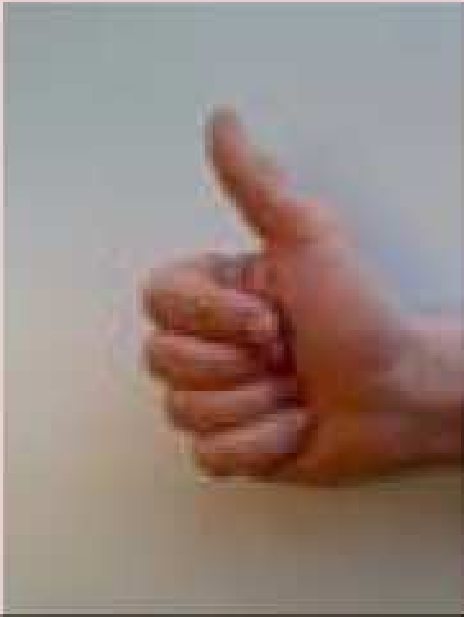
\includegraphics[width=\linewidth]{./img/moves/mov1.png} &
		2	&	Extensão do indicador e dedo médio, flexão dos outros dedos.	& 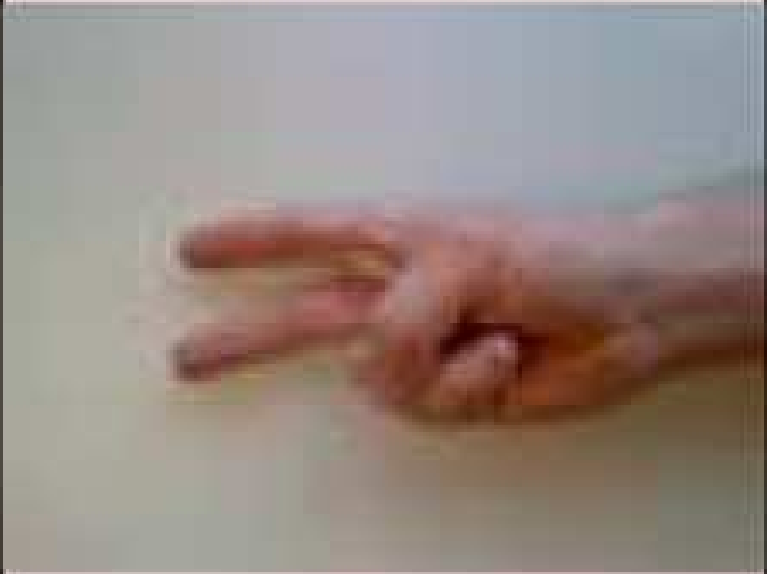
\includegraphics[width=\linewidth]{./img/moves/mov2.png} &
		3	&	Flexão do dedo anelar e mínimo, extensão dos outros dedos.	& 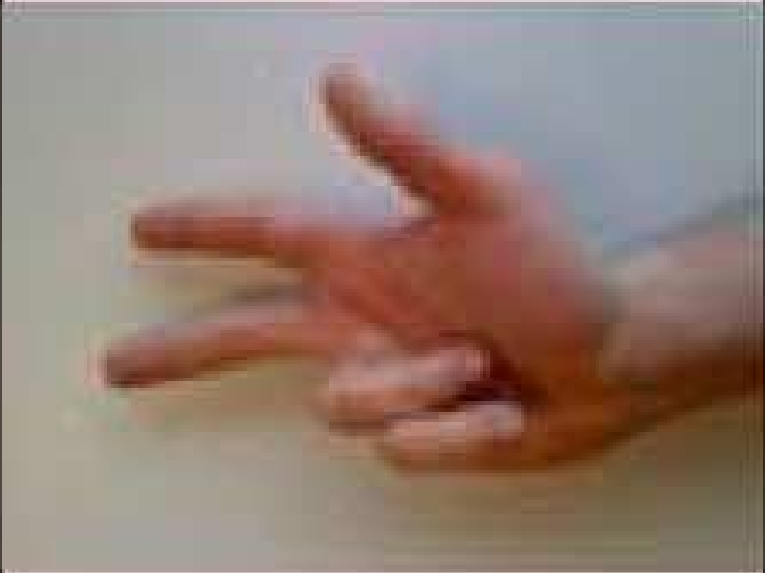
\includegraphics[width=\linewidth]{./img/moves/mov3.png}\\
		\midrule
		4	&	Polegar para a base do dedo mínimo.	& 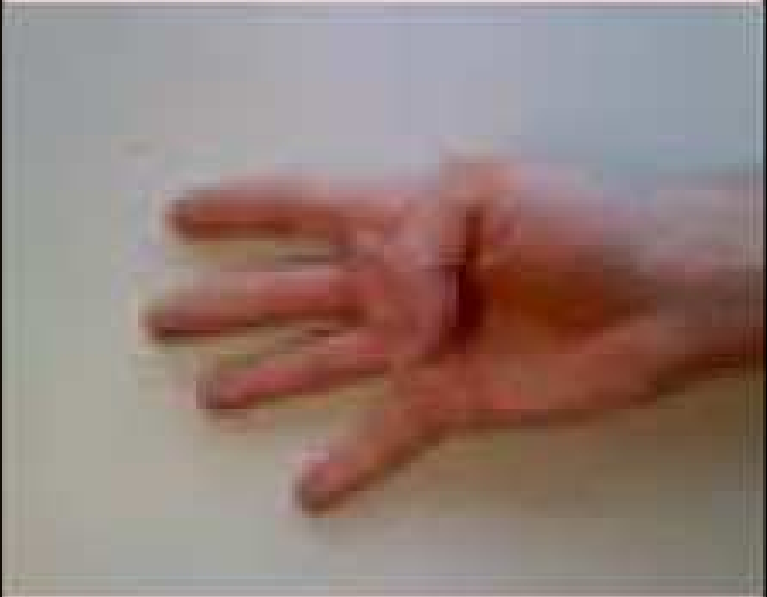
\includegraphics[width=\linewidth]{./img/moves/mov4.png} &
		5	&	Abdução (``afastamento'') de todos os dedos extendidos.	& 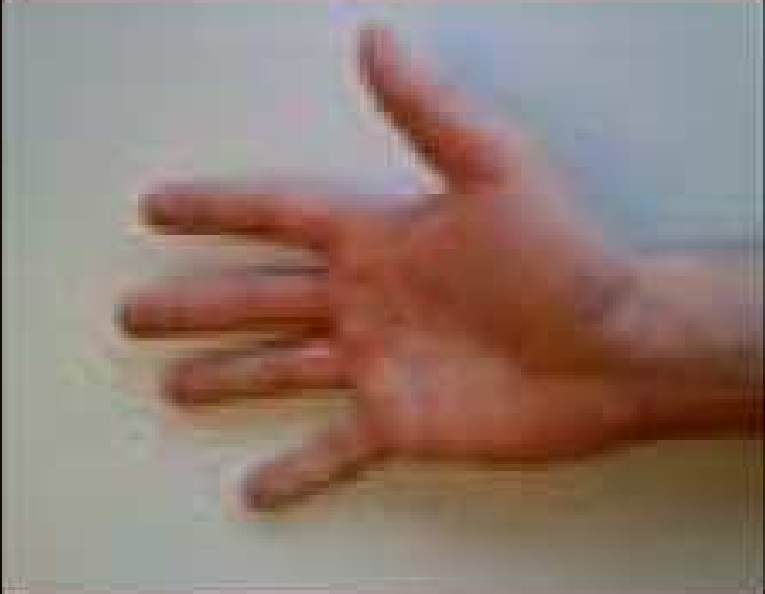
\includegraphics[width=\linewidth]{./img/moves/mov5.png} &
		6	&	Flexão de todos os dedos ao punho.	& 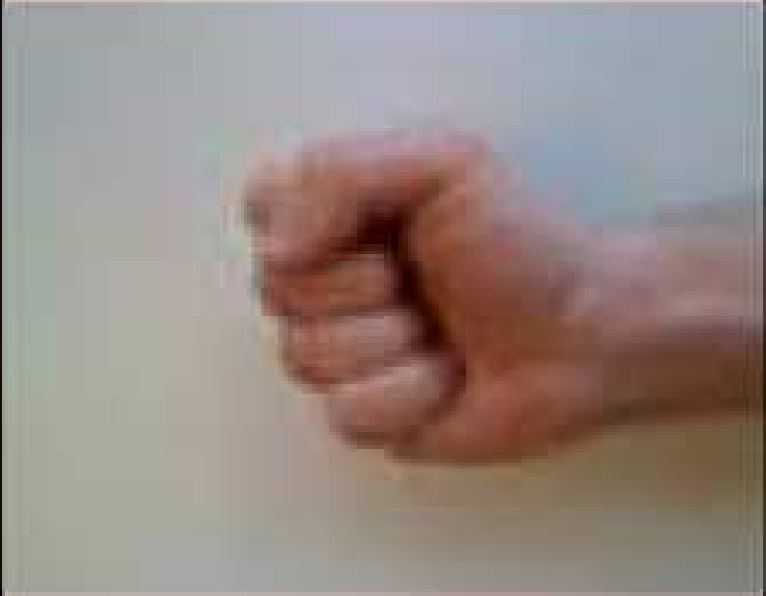
\includegraphics[width=\linewidth]{./img/moves/mov6.png}\\
		\midrule
		7	&	Extensão do indicador em movimento de ``apontar''.	& 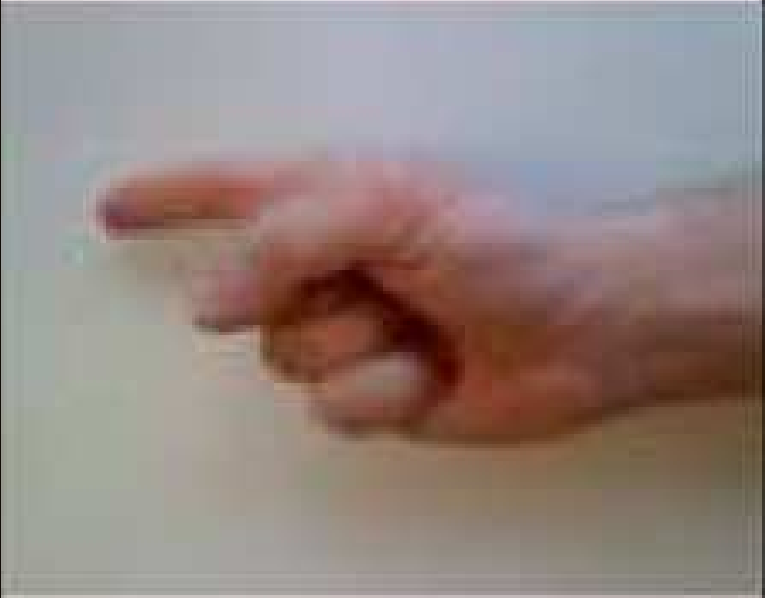
\includegraphics[width=\linewidth]{./img/moves/mov7.png} &
		8	&	Adução (``aproximação'') de todos os dedos extendidos.	& 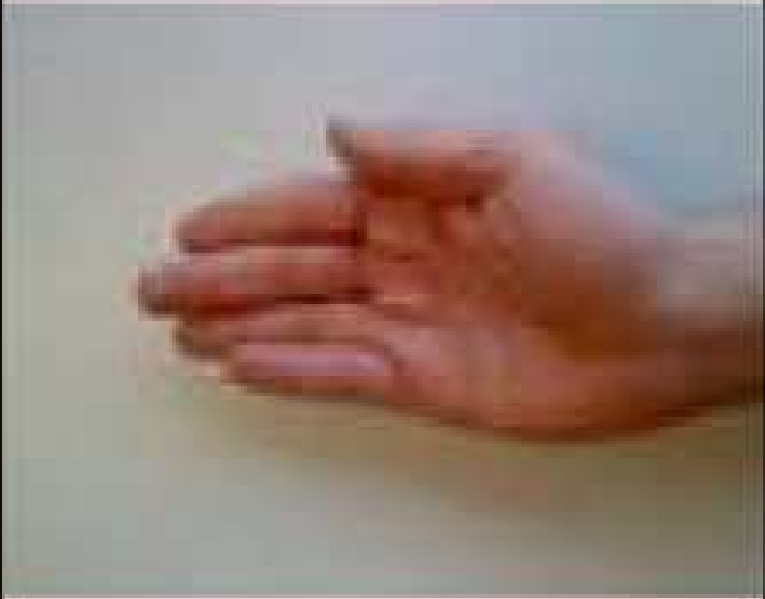
\includegraphics[width=\linewidth]{./img/moves/mov8.png} &
		9 10	&	Rotação de punho em torno do dedo médio, dois sentidos.	& 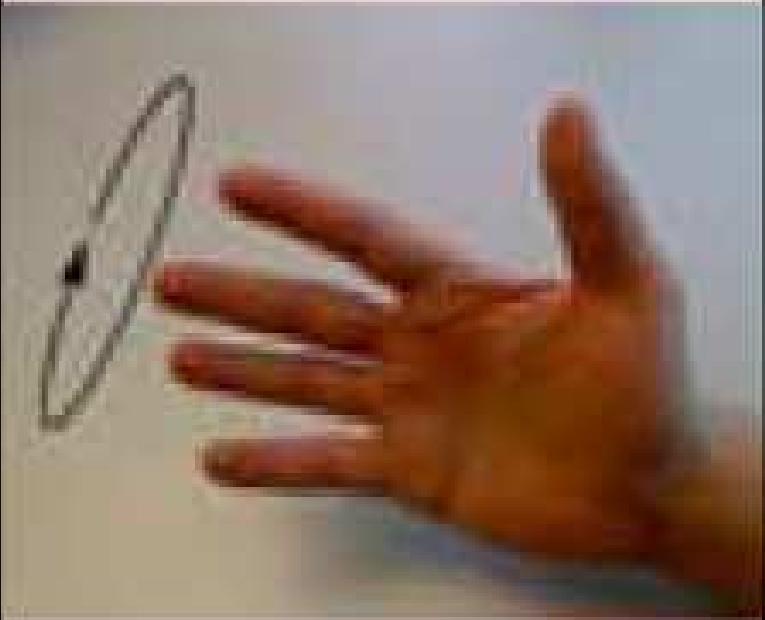
\includegraphics[width=\linewidth]{./img/moves/mov9.png} 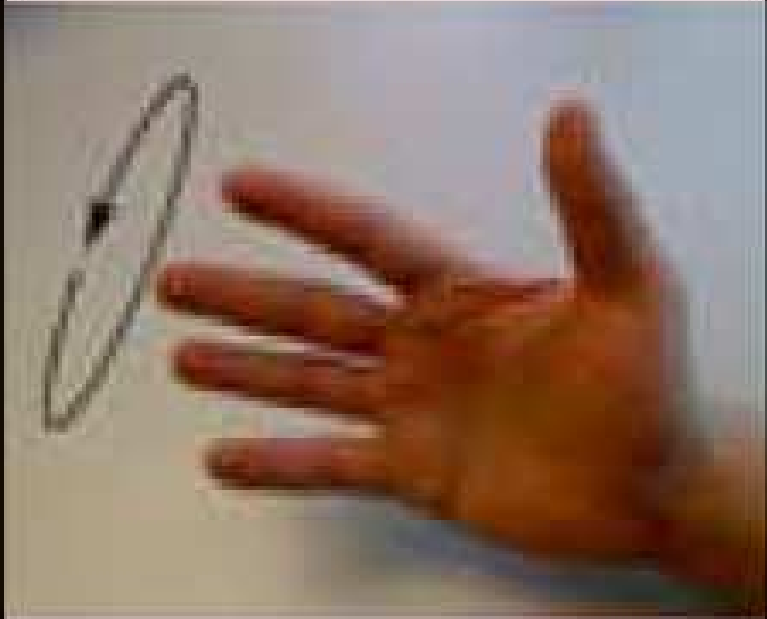
\includegraphics[width=\linewidth]{./img/moves/mov10.png} \\
		\midrule
		11 12	&	Rotação de punho em torno do dedo mínimo, dois sentidos.	& 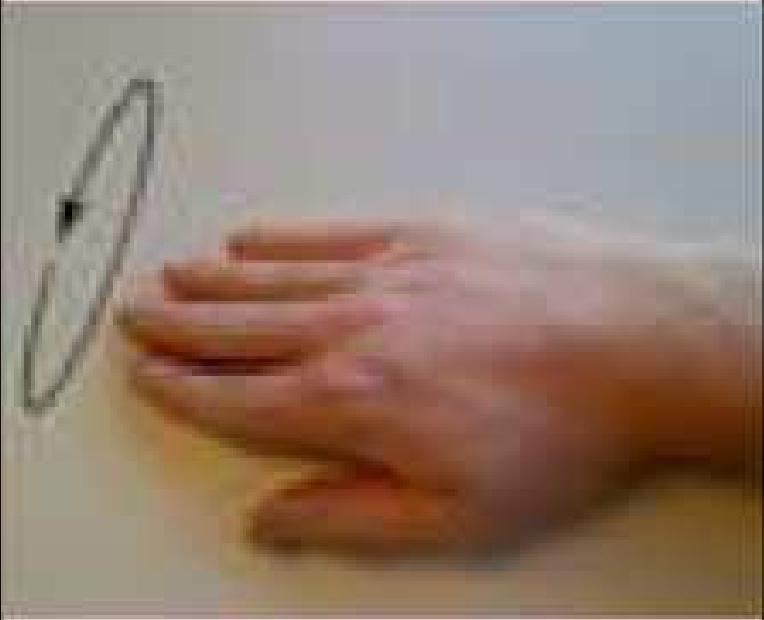
\includegraphics[width=\linewidth]{./img/moves/mov11.png} 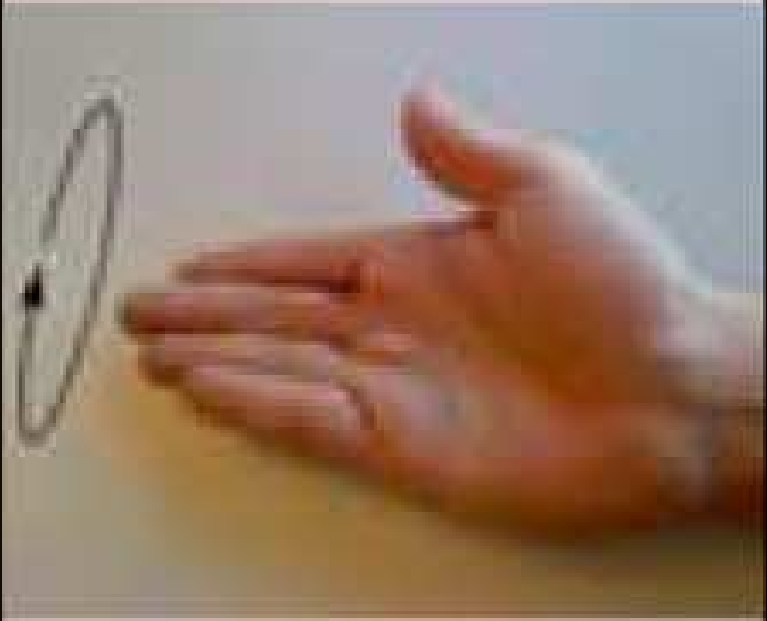
\includegraphics[width=\linewidth]{./img/moves/mov12.png} &
		13	&	Flexão de punho.	& 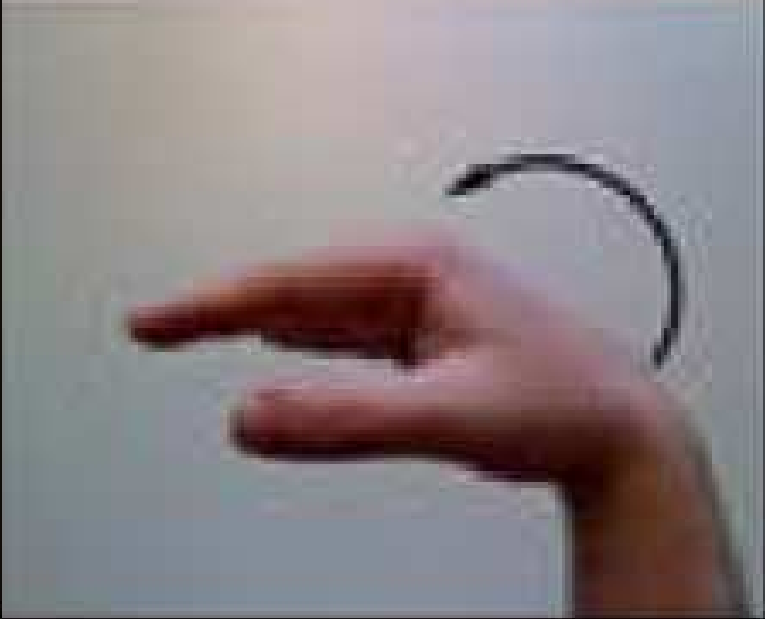
\includegraphics[width=\linewidth]{./img/moves/mov13.png} &
		14	&	Extensão de punho.	& 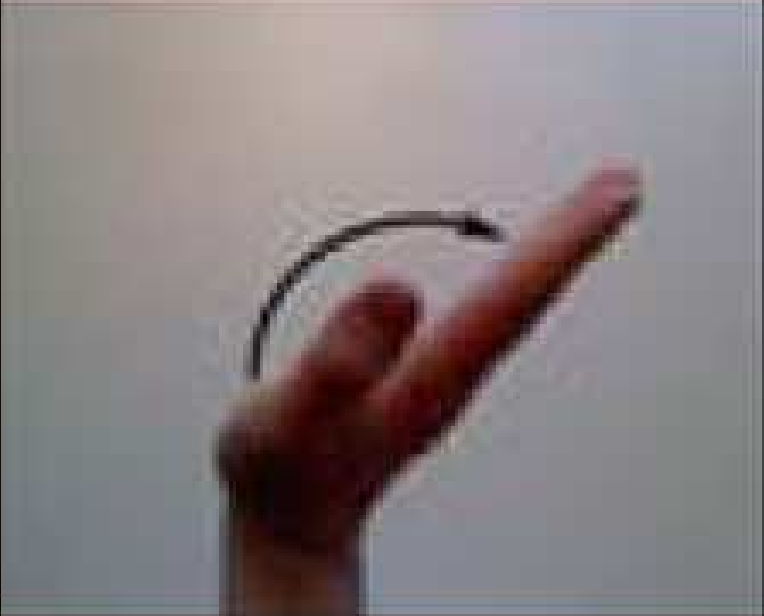
\includegraphics[width=\linewidth]{./img/moves/mov14.png}\\
		\midrule
		15	&	Desvio radial do punho.	& 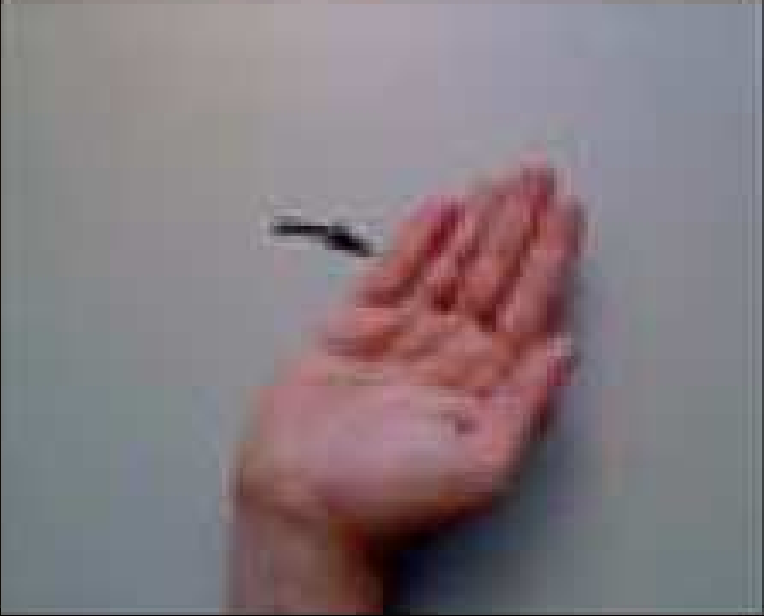
\includegraphics[width=\linewidth]{./img/moves/mov15.png} &
		16	&	Desvio ulnar do punho.	& 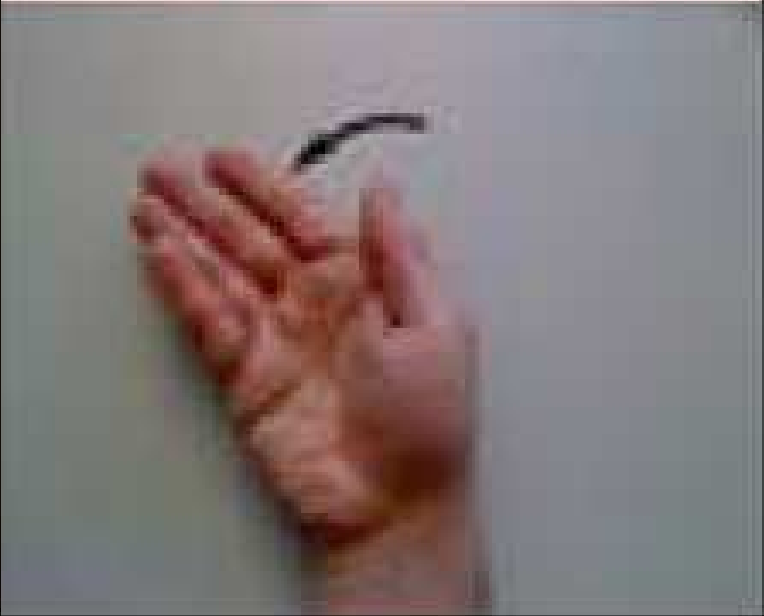
\includegraphics[width=\linewidth]{./img/moves/mov16.png} &
		17	&	Extensão de punho com mão cerrada.	& 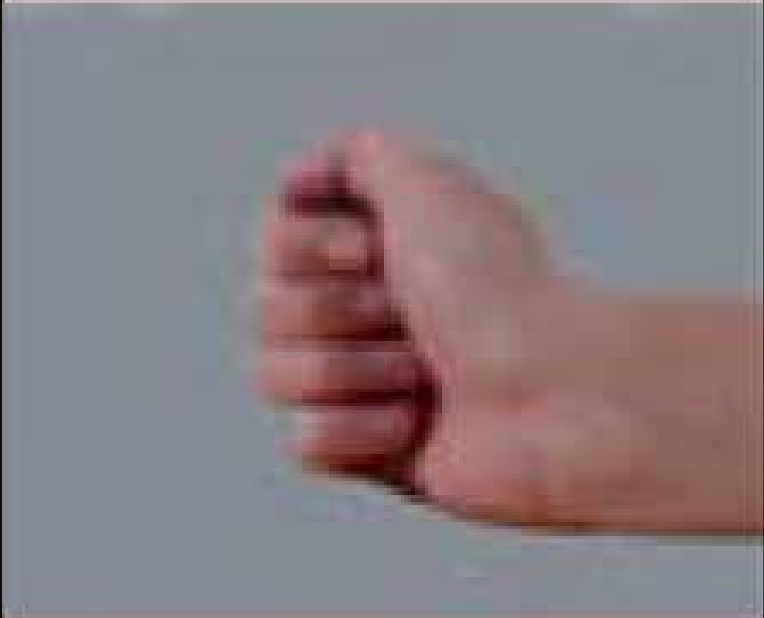
\includegraphics[width=\linewidth]{./img/moves/mov17.png}\\
		\bottomrule
	\end{tabular}
\end{table}
